\documentclass[titlepage]{article}

\usepackage[utf8]{inputenc}
\usepackage{csvsimple}
\usepackage{amsmath, amssymb, amsthm}
\usepackage{graphicx, float}
\usepackage{caption}
\usepackage{subcaption}

\usepackage[top=1.0in, bottom=1.0in, left=1.20in, right=1.20in]{geometry}
\graphicspath{{images/}}

\usepackage[
backend=biber,
style=authoryear,
sorting=ynt
]{biblatex}

\addbibresource{references.bib}

\title{%
Lab Report 3: \\ Acceleration Due to Gravity \\



}
\author{
\large Author: Jeff Khuu \\
CCID: khuu1 \\
Lab Partner(s): Harsh Brar \\
PHYS 144, LAB-DW21
}
\date{Date of Lab: September 24, 2025}

\begin{document}
\maketitle
\section{Results}

Linearized equations for the curve of best fit and line of best fit can be found using the following kinematics equations for a constant acceleration due to gravity, $g$,
$$ y = \underbrace{-\frac{1}{2}gt^2}_{ax^2} + \underbrace{v_{0y}t}_{bx} + \underbrace{y_0}_{c}  $$
$$ \underbrace{v}_{y} = \underbrace{-gt}_{mx} - \underbrace{v_{0y}}_{b} $$
Using a computer algorithm to generate the parameters of each polynomial fit and covariant matrix,
the acceleration due to gravity and initial velocity for each equation can be found using the following relationships:
\begin{equation}\label{eq:curve-acceleration}
   \begin{split}
      a & = -\frac{1}{2}g \\
      g & = -2a
   \end{split} 
\end{equation}

\begin{equation}\label{eq:slope}
   \begin{split}
      m &= -g \\
      g &= -m
   \end{split}
\end{equation}

\begin{equation}\label{eq:slope-initial_velocity}
   \begin{split}
      b &= -{v_0y} \\
      v_{0y} &= -b
   \end{split}
\end{equation}
Computing each parameter using the complete data from Table \ref{tab:truncated-data} yields the following values,

The value given by Eq.\ref{eq:curve-acceleration} yields $g = 9.83\pm 0.18 m/s^2$. 

The value given by Eq.\ref{eq:slope} yields the value $g = 9.65\pm0.45m/s^2$

The value given by Eq.\ref{eq:slope-initial_velocity} yields $v_{0y} = 0.926\pm0.102m/s$


\begin{table}[h]
   \caption{Estimated height and velocity of a tennis ball in freefall. Origin at the starting position of the tennis ball with a negative downwards direction. Velocity calculated by Tracker. Full data can be found in the Appendix.}
   \label{tab:truncated-data}
   \begin{center}
      \csvautotabular{phys144lab3-data-truncated.csv}
   \end{center}
\end{table}

\begin{figure}[H]
   \begin{center}
      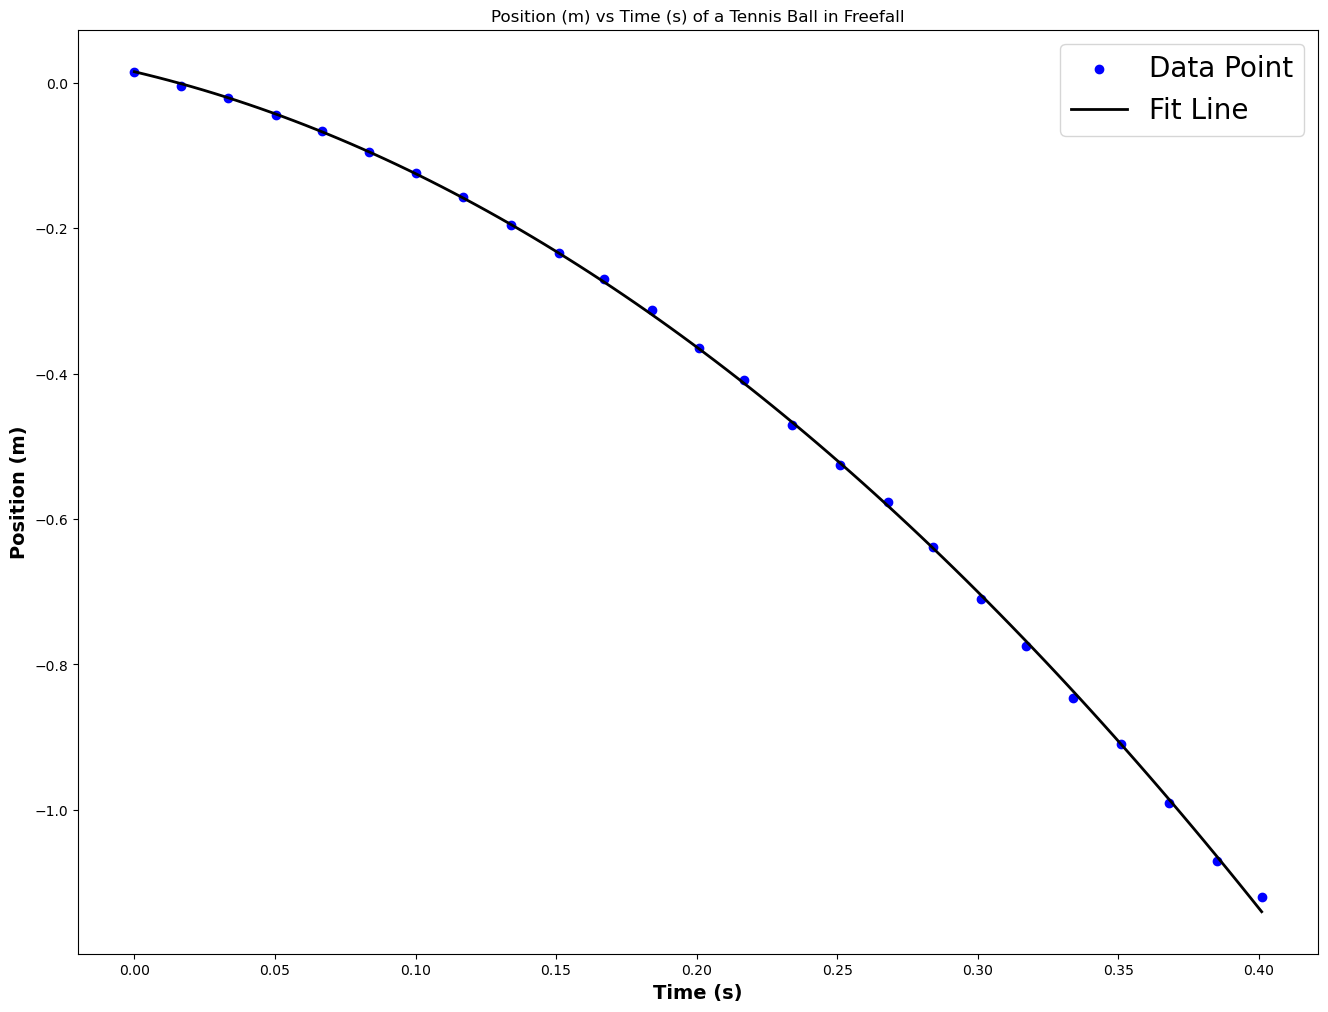
\includegraphics[width=0.8\textwidth]{phys144lab3-position_time_graph.png} 
   \end{center}
   \caption{Graph of the position vs. time of a tennis ball in freefall. Computed curve of best fit shown by solid black line. Fit parameter, $a$ can be used to compute the experimental value, see Eq.\ref{eq:curve-acceleration}.}
\end{figure}

\begin{figure}[H]
   \begin{center}
      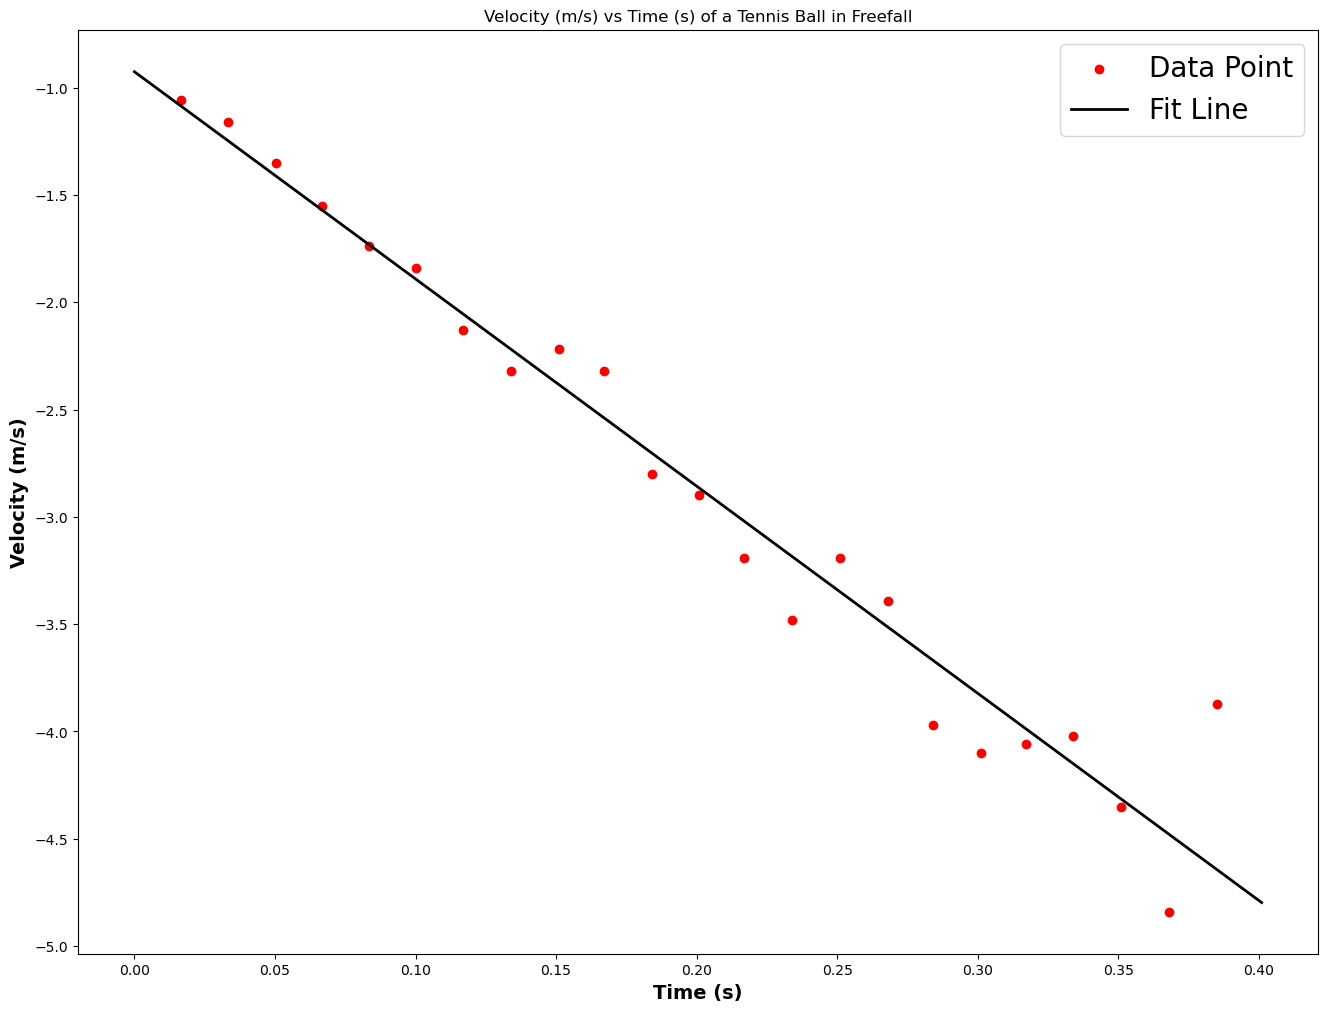
\includegraphics[width=0.8\textwidth]{phys144lab3-velocity_time_graph.png} 
   \end{center}
   \caption{Graph of the velocity vs. time of a tennis ball in freefall. Computed line of best fit shown by solid black line. Slope and intercept can be used to compute experimental values, see Eq. \ref{eq:slope} and \ref{eq:slope-initial_velocity} }
\end{figure}

\section{Discussion}
The experimental value for the acceleration due to gravity of the velocity-time graph is $9.65\pm0.45 m/s^2$. 
Since the theoretical acceleration due to gravity is defined as $g = 9.81m/s^2$,
our experimentally determined value is within one interval of uncertainty and is agreeance with the expected value.
The result is 98.4\% of the theoretical value.

The experimental value for the initial velocty $v_{0y}$ of the tennis ball in freefall using the velocity-time graph is $0.926\pm0.102m/s$.
Since the tennis ball is being dropped from rest we expect the value of $v_{0y}$ to be 0m/s. 
The experimentally determined value is more than 9 intervals of uncertainty from the expected value and is disagreeance with the theoretical value.

In general, the curve and line of best represent the data points well. The most inconsistent data points occur near the end of freefall when the ball comes closer to hitting the ground. 
Removing outlying points and reanalyzing would have the effect of increasing our experimental value of $g$ (for example by steepening the curve of the velocity-time graph.) Resulting in bringing the experimental and theoretical values closer together.

The human factor plays an important role in completing video analysis. My lab partner obtained the experimental value $g = 9.82\pm0.15m/s^2$ when analyzing their position-time graph but obtained the value
$g = 11.63\pm0.89m/s^2$ and $v_{0y} = 1.21\pm0.16m/s$ when analyzing their velocity-time graph despite having the same video data. While most of their values are in agreeance with my experimentally determined values, the value of $g$ found using the velocity-time graph is in poor agreenace with my result and with the theoretical value.
Factors such as motion blur in the video and differences in personal judgement in terms of placing origins and calibrating distances could cause experimental values to deviate from one another despite using the same original video data.

The inconsistent experimental value of $v_{0y}$ could be caused by accidentally imparting an initial velocity when dropping the ball from height. Furthermore, an inconsistent placement of origin
that does not exactly reflect the balls starting position when plotting points in Tracker could result in a perceived initial velocity when doing analysis. 

A potential improvement to the procedure of the experiment could be to roll the tennis ball off a level table to ensure that there is no initial downwards velocity. This change would not affect the acceleration due to gravity because the x and y components of position do not affect each other.
Another improvement could be to ensure the alignment of the calibration meter stick to be perpendicular to the ground and vertically parallel to the recording device. As well as aligning to be in the same horizontal plane of motion as the falling tennis ball.
This can be achieved by rolling the tennis ball off a table with the calibration stick fixed to the leg of the table or using a stand to vertically align the calibration stick without needing to prop it up or lean it against another object.
The effect of these changes would improve the accuracy of the data used in analysis resulting in experimental values closer to the theoretical value.

\newpage

\section{References and Acknowledgements}

\nocite{*}
\printbibliography

I would like to acknowledge Harsh Brar, my lab partner for helping setup and collect data for the lab and allowing me to use his calculated experimental values for comparison in my Disussion.

\section{Appendix}

\begin{table}[h]
   \caption{Full data table of estimated height and velocity of a tennis ball in freefall. Origin at the starting position of the tennis ball with a negative downwards direction. Velocity calculated by Tracker.}
   \label{tab:complete-data}
   \begin{center}
      \csvautotabular{phys144lab3-data-complete.csv}
   \end{center}
\end{table}

\end{document}
